%
\subsection{Lexical versus abstract contexts}
\label{sec:contexts}

We would like to further analyze the kinds of linguistic features that the
hidden dimensions of RNNs encode. Previous work  
\cite{karpathy2015visualizing,li2015convergent} has shown that in response 
to the task the networks are trained for, individual dimensions in the hidden layers of 
RNNs can become {\it specialised} in responding to certain types of triggers, including 
the tokens or token types at each time step, as well as the preceding context of
each token in the input sentence.

Here we perform a further comparison between the models based on the hypothesis 
that due to their different objectives, the activations of the dimensions of the last 
hidden layer of {\sc Visual} are more characterized by semantic relations within 
contexts, whereas the hidden dimensions in {\sc Textual} and {\sc LM} are 
more focused on extracting syntactic patterns. In order to quantitatively test this 
hypothesis, we measure the strength of association between activations of hidden 
dimensions and either lexical (token n-grams) or structural (dependency label n-grams) types 
of context. 

For each pathway, we define $A_i$ as a discrete random variable corresponding 
to a binned activation over time steps at hidden dimension $i$, and $C$ 
as a discrete random variable indicating the context 
(where $C$ can be of type `word trigram' or `dependency label bigram', for example). 
The strength of association between $A_i$ and $C$ can be measured 
by their mutual information:
\begin{equation}
\mathrm{I}(A_i;C) = \sum_{a\in{A_i}}\sum_{c\in{C}} p(a,c)\log\left(\frac{p(a,c)}{p(a)p(c)}\right) 
\end{equation}
Similarly to \namecite{li2015convergent}, the activation value
distributions are discretized into percentile bins per dimension, such
that each bin contains 5\% of the marginal density. For context types,
we used unigrams, bigrams and trigrams of both dependency labels and
words. Figure~\ref{fig:raw_mutual} shows the distributions of the
mutual information scores for the three networks and the six context
types. Note that the scores are not easily comparable between context
types, due the different support of the distributions; they are,
however, comparable across the networks. The figure shows {\sc LM} and
{\sc Textual} as being very similar, while {\sc Visual} exhibits a
different distribution. We next compare the models' scores pairwise to
pinpoint the nature of the differences.
\begin{figure}
  \centering
  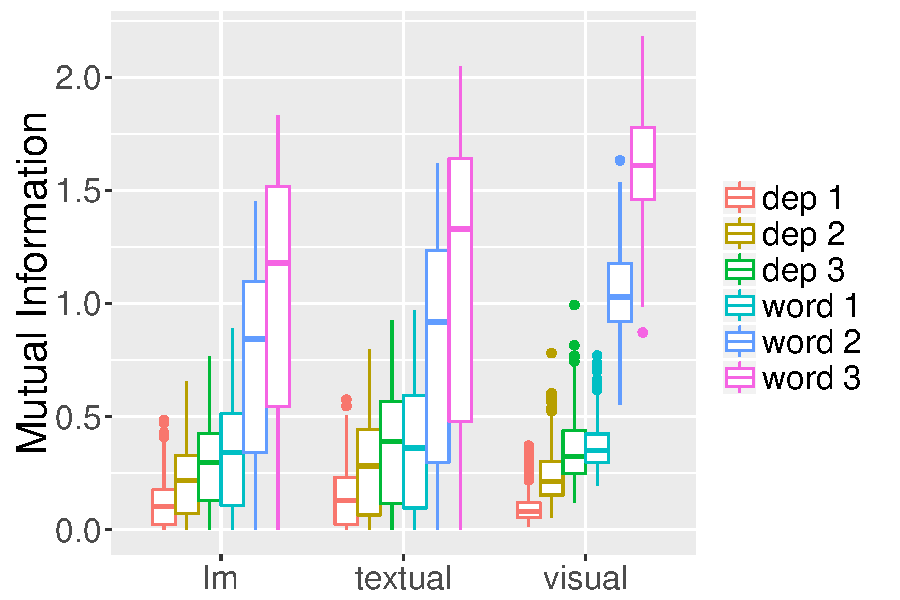
\includegraphics[scale=0.6]{raw_mutual.pdf}
  \caption{Distributions of the mutual information scores for the three networks and the six context types.}
  \label{fig:raw_mutual}
\end{figure}

We use the notation $\mathrm{MI}^\mathit{LM}_C$,  $\mathrm{MI}^T_C$ and  $\mathrm{MI}^V_C$ 
to denote the median mutual information score over all dimensions of {\sc LM}, {\sc Textual} and {\sc Visual} 
respectively, when considering context $C$. 
We then compute log ratios $\log(\mathrm{MI}^{T}_{C}/\mathrm{MI}^{V}_{C})$ and $\log(\mathrm{MI}^\mathit{LM}_{C}/\mathrm{MI}^{T}_{C})$
for all six context types $C$. In order to quantify variability we bootstrap this statistic with
5000 replicates. Figure~\ref{fig:mi-boot} shows the resulting bootstrap distributions 
for uni-, bi-, and trigram contexts, in the word and dependency conditions. 


The clear pattern is that for {\sc Textual} versus {\sc Visual}, the
log ratios are much higher in the case of the dependency contexts,
with no overlap between the bootstrap distributions. Thus, in general,
the size of the relative difference between {\sc Textual} and {\sc
  Visual} median mutual information score is much more pronounced for
dependency context types.  This suggests that features that are
encoded by the hidden dimensions of the models are indeed different, and
that the features encoded by {\sc Textual} are more associated with
syntactic constructions than in the case of {\sc Visual}. In contrast,
when comparing {\sc LM} with {\sc Textual}, the difference between
context types is much less pronounced, with distributions
overlapping. Though the difference is small, it goes in the direction
of the dimensions of the {\sc Textual} model showing higher
sensitivity towards dependency contexts.

\begin{figure}
  \centering
  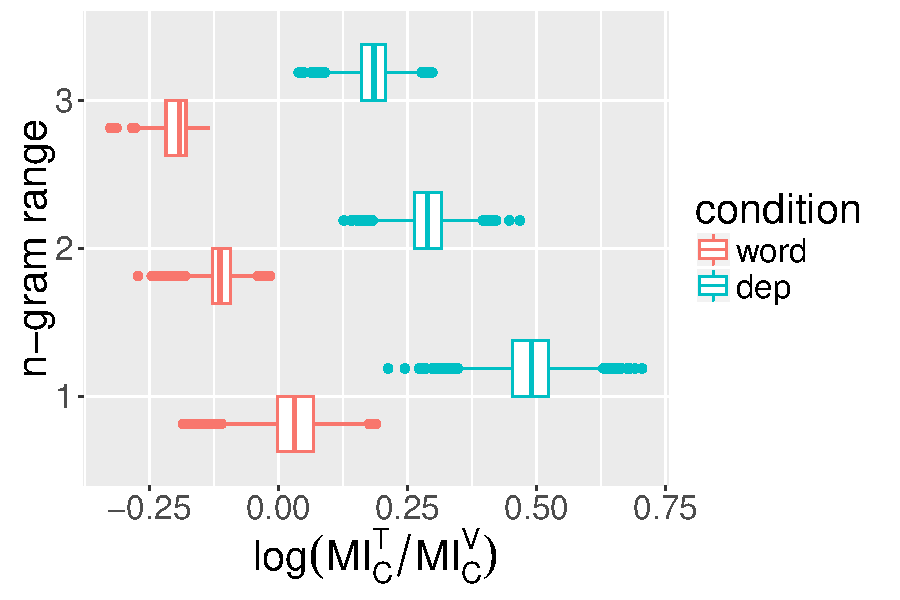
\includegraphics[scale=0.4]{bootstrappedMI.pdf}
  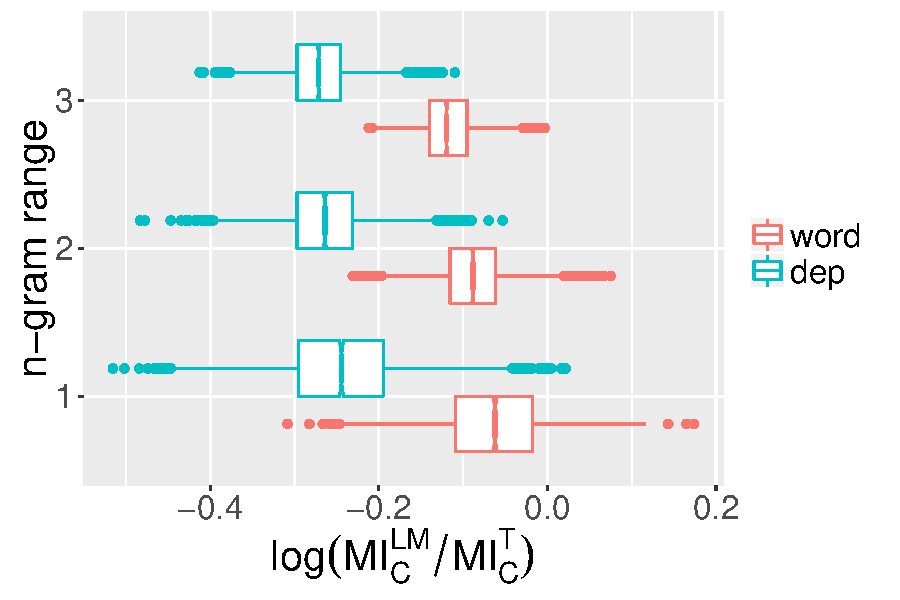
\includegraphics[scale=0.4]{bootstrappedMI2.pdf}
  \caption{Bootstrap distributions of log ratios of median mutual
    information scores for word and dependency contexts. Left: {\sc Textual}
      vs {\sc Visual}; right: {\sc LM} vs {\sc Textual}}
  \label{fig:mi-boot}
  \vspace{-.2cm}
\end{figure}


The mutual information scores can be used to pinpoint specific
dimensions of the hidden activation vectors which are strongly
associated with a particular type of
context. Table~\ref{tab:mi-examples} lists for each network the
dimension with the highest mutual information score with respect to
the {\it dependency trigram} context type, together with the top
five contexts where these dimensions carry the highest value. In spite
of the quantitative difference between the networks discussed above,
the dimensions which come up top seem to be capturing something quite
similar for the three networks: (a part of) a construction with an
animate root or subject modified by a participle or a prepositional
phrase, though this is somewhat less clean-cut for the {\sc Visual}
pathway where only two out of five top context clearly conform to this
pattern.  Other interesting templates can be found by visual
inspection of the contexts where high-scoring dimensions are active;
for example, dimension 324 of {\sc LM} is high for {\it word bigram} 
contexts including
{\it people preparing, gets ready, man preparing, woman preparing,
  teenager preparing}.

\begin{table}
  \centering
  \caption{Dimensions most strongly associated with the dependency trigram context type, and the top five contexts in which these dimensions have high values.} 
\label{tab:mi-examples}
\begin{tabular}{lll}
  Network            & Dimension & Examples         \\\hline
  {\sc LM}           & 511       & cookie/pobj attached/acl to/prep \\
                     &           & people/pobj sitting/acl in/prep \\
                     &           & purses/pobj sitting/pcomp on/prep\\
                     &           & and/cc talks/conj on/prep \\
                     &           & desserts/pobj sitting/acl next/advmod \\\hline
  {\sc Textual}      & 735       & male/root on/prep a/det        \\
                     &           & person/nsubj rides/root a/det   \\
                     &           & man/root carrying/acl a/det \\
                     &           & man/root on/prep a/det         \\
                     &           & person/root on/prep a/det       \\\hline
  {\sc Visual}       &  875      & man/root riding/acl a/det \\
                     &           & man/root wearing/acl a/det \\
                     &           & is/aux wearing/conj a/det \\
                     &           & a/det post/pobj next/advmod \\
                     &           & one/nummod person/nsubj is/aux \\
\end{tabular}
\end{table}
